\documentclass{article}
\usepackage{amsmath,amssymb}
\usepackage{listings}
\usepackage{tikz}

\lstset{
  language=lean,
  basicstyle=\ttfamily\footnotesize,
  keywordstyle=\bfseries,
  breaklines=true,
  mathescape=true,
  escapeinside={(*}{*)},
  keepspaces=true
}

\begin{document}

\title{Issue XXIX: Comprehension Categories}
\author{Namdak Tonpa}
\date{}


\maketitle

\begin{abstract}
Comprehension categories provide a powerful categorical framework for modeling dependent
type theories, bridging the gap between categorical logic, topos theory, and type-theoretic
semantics. This paper presents a unified theoretical framework for comprehension categories,
offering precise definitions, key theorems, and novel applications.

We define a comprehension
category as a category $\mathcal{C}$
equipped with a fibration $p: \mathcal{E} \to \mathcal{C}$
and a comprehension map that assigns to each type $A \in \mathcal{E}A \in \mathcal{E}$
over a context $\Gamma \in \mathcal{C}$
an extended context $\Gamma.A \in \mathcal{C}$,
satisfying pullback stability. We introduce variants, including split and
non-split comprehension categories, and contextual categories, to accommodate
strict and non-strict type theories. Key theorems include the equivalence theorem,
establishing that every comprehension category induces a model of dependent type theory,
and the splitting theorem, demonstrating that any comprehension category can be replaced
by an equivalent split comprehension category. We further explore the relationship
between comprehension categories and related structures, such as Categories with
Representations (CwR) and Categories with Families (CwF), highlighting their
functorial and computational interpretations. Applications are presented in
categorical semantics, homotopy type theory, and topos theory, including the
interpretation of univalence axioms and the construction of syntactic categories.
This framework unifies existing approaches, clarifies the categorical
underpinnings of dependent types, and paves the way for future developments
in type-theoretic and geometric foundations of mathematics.

As instantiation example we present a categorical model of Martin-Löf Type Theory (MLTT-75)
with dependent products ($\Pi$-types), dependent sums ($\Sigma$-types),
and identity types (Id-types) using Comprehension Categories.
The model uses a comprehension category, a Grothendieck fibration
with a comprehension functor, to capture type dependency and context extension.
Formal definitions are provided, with pullback diagrams resembling Awodey’s natural models.
\end{abstract}

\ifincludeTOC
  \tableofcontents
\fi

\section{Comprehension Categories}
Martin-Löf Type Theory (MLTT-75) is a dependent type theory with $\Pi$-types, $\Sigma$-types, and Id-types. Its categorical semantics is often modeled using Grothendieck fibrations, with comprehension categories providing a structured framework for type dependency and context extension \cite{ncatlab, jacobs1993}. We formalize a model using a comprehension category, based on a split Grothendieck fibration with a comprehension functor, inspired by the codomain fibration. The model is implemented in Lean 4 without dependencies, ensuring a minimal presentation. Pullback diagrams, styled after Awodey’s natural models \cite{awodey}, illustrate the type formers, with constructors (e.g., $\lambda$, pair, refl) on upper arrows and type formers on lower arrows.

\newpage
\subsection{Definitions}
A split Grothendieck fibration $p : \mathcal{E} \to \mathcal{B}$ models dependent types, with functorial Cartesian lifts for strict substitution.


\begin{definition}[Cleavage]
A \emph{cleavage} for a Grothendieck fibration \(p : \mathcal{E} \to \mathcal{C}\) assigns
to each \(e \in \mathcal{E}\) and \(f : c' \to p(e)\) in \(\mathcal{C}\) a Cartesian
morphism \(\phi_f : f^*e \to e\) in \(\mathcal{E}\) such that \(p(\phi_f) = f\), where \(f^*e \in \mathcal{E}_{c'}\).
\end{definition}

\begin{definition}[Split Fibration 1]
A Grothendieck fibration \(p : \mathcal{E} \to \mathcal{C}\) is
a \emph{split fibration} if it has a cleavage such that the
assignment \(f \mapsto f^*e\) defines a functor \(f^* : \mathcal{E}_{p(e)} \to \mathcal{E}_{c'}\)
for each fiber category \(\mathcal{E}_c\), and \((g \circ f)^* = f^* \circ g^*\).
\end{definition}

\begin{definition}[Split Fibration 2]
A \emph{split fibration} $p : \mathcal{E} \to \mathcal{B}$ is a functor $p$ with:
\begin{itemize}
  \item For every $e \in \mathcal{E}.\text{Ob}$ and $f : b' \to p(e)$ in $\mathcal{B}$, a chosen lift $(e', \phi : e' \to e)$ with $p(\phi) = f$.
  \item Uniqueness: For any two lifts $(e_1, \phi_1)$, $(e_2, \phi_2)$ with $p(\phi_1) = p(\phi_2) = f$, there exists $\chi : e_2 \to e_1$ with $p(\chi) = \text{id}$ and $\phi_1 \circ \chi = \phi_2$.
\end{itemize}
\end{definition}

\begin{lstlisting}[mathescape=true]
structure SplitFibration (E B : Category) where
  functor : Functor E B
  lift : $\forall$ {e : E.Ob} {b' : B.Ob} (f : B.Hom b' (functor.obj e)),
    (e' : E.Ob) $\times$ (phi : E.Hom e' e) $\times$ (functor.map phi = f)
  lift_unique : $\forall$ {e : E.Ob} {b' : B.Ob} (f : B.Hom b' (functor.obj e))
    (e1 e2 : E.Ob) (phi1 : E.Hom e1 e) (phi2 : E.Hom e2 e),
    functor.map phi1 = f $\to$ functor.map phi2 = f $\to$
    $\exists$ (chi : E.Hom e2 e1), functor.map chi = B.id $\wedge$ E.comp phi1 chi = phi2
\end{lstlisting}

\begin{definition}[Arrow Category]
The \emph{arrow category} \(\mathcal{C}^\to\) of a category \(\mathcal{C}\) has:
\begin{itemize}
    \item Objects: Morphisms \(f : A \to B\) in \(\mathcal{C}\).
    \item Morphisms: From \(f : A \to B\) to \(g : C \to D\), a pair \((h_1 : A \to C, h_2 : B \to D)\) such that \(g \circ h_1 = h_2 \circ f\).
    \item Composition: For \((h_1, h_2) : f \to g\) and \((k_1, k_2) : g \to l\), the composite is \((k_1 \circ h_1, k_2 \circ h_2)\).
\end{itemize}
\end{definition}

\begin{definition}[Comprehension Functor]
For a split fibration \(p : \mathcal{E} \to \mathcal{C}\), a \emph{comprehension functor} is a functor \(\{-\} : \mathcal{E} \to \mathcal{C}^\to\) that maps each object \(A \in \mathcal{E}\) to a morphism \(\pi : \Gamma' \to p(A)\) in \(\mathcal{C}\), and each morphism \(f : A \to B\) in \(\mathcal{E}\) to a morphism \((h_1, h_2) : \{A\} \to \{B\}\) in \(\mathcal{C}^\to\).
\end{definition}

\begin{definition}[Comprehension Category]
A \emph{comprehension category} consists of:
\begin{itemize}
    \item A split fibration \(p : \mathcal{E} \to \mathcal{C}\).
    \item A terminal object \(T \in \mathcal{C}\).
    \item A comprehension functor \(\{-\} : \mathcal{E} \to \mathcal{C}^\to\), mapping \(A \in \mathcal{E}\) to \((\Gamma', \pi : \Gamma' \to p(A))\).
    \item An adjunction: For \(\sigma : \Delta \to \Gamma\) in \(\mathcal{C}\) and \(A \in \mathcal{E}_\Gamma\), there exists \(A' \in \mathcal{E}_\Delta\) with \(p(A') = \Delta\) and a morphism \(f : A' \to A\) such that \(p(f) = \sigma\).
\end{itemize}
\end{definition}

\begin{definition}[Comprehension Category]
A comprehension category models MLTT-75 with a fibration and a comprehension functor for context extension.
A \emph{comprehension category} consists of:
\begin{itemize}
  \item A split fibration $p : \mathcal{E} \to \mathcal{B}$.
  \item A terminal object $T \in \mathcal{B}.\text{Ob}$.
  \item A comprehension functor $\{-\} : \mathcal{E} \to \mathcal{B}^\to$, mapping $A \in \mathcal{E}$ to $(\Gamma', \pi : \Gamma' \to p(A))$.
  \item An adjunction: For $\sigma : \Delta \to \Gamma$ and $A \in \mathcal{E}_\Gamma$, there exists $A' \in \mathcal{E}_\Delta$ with $p(A') = \Delta$ and a morphism $f : A' \to A$ such that $p(f) = \sigma$.
  \item Pullbacks in $\mathcal{B}$ for context extension.
  \item Structure for $\Pi$-types (fiber exponentials), $\Sigma$-types (composition), and Id-types (diagonals).
\end{itemize}
\end{definition}

\begin{definition}[Beck-Chevalley Condition]
Let \(p : \mathcal{E} \to \mathcal{C}\) be a fibration, and consider a pullback square in \(\mathcal{C}\):
\[
\begin{CD}
\Delta @>q>> \Gamma' \\
@V h VV @VV g V \\
\Gamma @>>f> \Theta
\end{CD}
\]
where \(f \circ h = g \circ q\). For a functor \(F : \mathcal{E}_{\Gamma'} \to \mathcal{E}_\Gamma\) with a left or right adjoint \(G : \mathcal{E}_\Gamma \to \mathcal{E}_{\Gamma'}\), the \emph{Beck-Chevalley condition} holds if the canonical natural transformation induced by the pullback, \(h^* \circ G \to q^* \circ F\) (for right adjoints) or \(q^* \circ F \to h^* \circ G\) (for left adjoints), is an isomorphism.
\end{definition}

\newpage



\begin{definition}[Dependent Sum]
In a comprehension category with
fibration \(p : \mathcal{E} \to \mathcal{C}\), a \emph{dependent sum} for
a type \(\sigma \in \mathcal{E}_\Gamma\) is
a functor \(\Sigma_\sigma : \mathcal{E}_{\Gamma.\sigma} \to \mathcal{E}_\Gamma\),
left adjoint to the substitution functor
\(p_\sigma^* : \mathcal{E}_\Gamma \to \mathcal{E}_{\Gamma.\sigma}\), such that for all morphisms \(f : \Delta \to \Gamma\) in \(\mathcal{C}\), the Beck-Chevalley condition holds, i.e., the canonical natural transformation \(\Sigma_{f^*\sigma} \circ q(f, \sigma)^* \cong f^* \circ \Sigma_\sigma\) is an isomorphism.
\end{definition}

\begin{definition}[Dependent Product]
In a comprehension category with fibration \(p : \mathcal{E} \to \mathcal{C}\), a \emph{dependent product} for a type \(\sigma \in \mathcal{E}_\Gamma\) is a functor \(\Pi_\sigma : \mathcal{E}_{\Gamma.\sigma} \to \mathcal{E}_\Gamma\), right adjoint to the substitution functor \(p_\sigma^* : \mathcal{E}_\Gamma \to \mathcal{E}_{\Gamma.\sigma}\), such that for all morphisms \(f : \Delta \to \Gamma\) in \(\mathcal{C}\), the Beck-Chevalley condition holds, i.e., the canonical natural transformation \(f^* \circ \Pi_\sigma \cong \Pi_{f^*\sigma} \circ q(f, \sigma)^*\) is an isomorphism.
\end{definition}

\begin{definition}[Identity Type]
In a split comprehension category with fibration \(p : \mathcal{E} \to \mathcal{C}\), an \emph{identity type} for a type \(\sigma \in \mathcal{E}_\Gamma\) consists of:
\begin{itemize}
    \item A type \(\mathrm{Id}_\sigma \in \mathcal{E}_{\Gamma.\sigma.\sigma}\), where \(\Gamma.\sigma.\sigma = p_\sigma^* \sigma\).
    \item A morphism \(r_\sigma : \Gamma.\sigma \to I_\sigma\), where \(I_\sigma = \Gamma.\sigma.\sigma.\mathrm{Id}_\sigma\), such that \(p_{\mathrm{Id}_\sigma} \circ r_\sigma = \mathrm{id}\).
    \item For any commutative square \(\langle f, M \rangle : \Delta \to \Gamma.\sigma\), \(\langle g, N \rangle : \Delta.\tau \to \Gamma.\sigma.\sigma\), a diagonal lifting \(h : I_\sigma \to \Delta.\tau\) making both triangles commute.
\end{itemize}
All data must be stable under substitutions.
\end{definition}

\begin{definition}[Category with Attributes]
A \emph{category with attributes} is a full split comprehension category, where the comprehension functor \(\{-\} : \mathcal{E} \to \mathcal{C}^\to\) is fully faithful, and types over \(\Gamma \in \mathcal{C}\) are determined by a functor \(\mathrm{Ty} : \mathcal{C}^{\mathrm{op}} \to \mathbf{Set}\).
\end{definition}

\begin{definition}[Display Map Category]
A \emph{display map category} is a comprehension category where the comprehension functor \(\{-\} : \mathcal{E} \to \mathcal{C}^\to\) is the inclusion of a full subcategory of \(\mathcal{C}^\to\), and all morphisms in the image are display maps.
\end{definition}

\begin{definition}[Contextual Category]
A \emph{contextual category} is a category with attributes equipped with:
\begin{itemize}
    \item A terminal object \(\bullet \in \mathcal{C}\).
    \item A length function \(\ell : \mathrm{obj}(\mathcal{C}) \to \mathbb{N}\) such that \(\ell(\bullet) = 0\), and for any type \(\sigma \in \mathcal{E}_\Gamma\), \(\ell(\Gamma.\sigma) = \ell(\Gamma) + 1\).
    \item For any non-empty context \(\Gamma\), a unique context \(\Delta\) (the father) and type \(\sigma \in \mathcal{E}_\Delta\) such that \(\Gamma = \Delta.\sigma\).
\end{itemize}
\end{definition}

\begin{definition}[Weakening Morphism]
In a comprehension category, a \emph{weakening morphism} is defined inductively:
\begin{itemize}
    \item A display map \(p_\sigma : \Gamma.\sigma \to \Gamma\) is a weakening morphism.
    \item If \(f : \Delta \to \Gamma\) is a weakening morphism and \(\sigma \in \mathcal{E}_\Gamma\), then \(q(f, \sigma) : \Delta.f^*\sigma \to \Gamma.\sigma\) is a weakening morphism.
\end{itemize}
\end{definition}

\begin{definition}[Variable]
In a comprehension category, for a type \(\sigma \in \mathcal{E}_\Gamma\), the \emph{variable} of type \(\sigma\) is the unique term \(v_\sigma : \Gamma.\sigma \to p_\sigma^* \sigma\) such that \(p_{p_\sigma^* \sigma} \circ v_\sigma = \mathrm{id}\).
\end{definition}

\begin{definition}[Universe]
In a split comprehension category with terminal object \(\bullet \in \mathcal{C}\), a \emph{universe} consists of:
\begin{itemize}
    \item A type \(\mathcal{U} \in \mathcal{E}_\bullet\), the context \(\bullet.\mathcal{U}\) also denoted \(\mathcal{U}\).
    \item A type \(\mathrm{El} \in \mathcal{E}_{\mathcal{U}}\), with context \(\mathcal{U}.\mathrm{El}\) denoted \(\widetilde{\mathcal{U}}\).
\end{itemize}
For a morphism \(f : \Gamma \to \mathcal{U}\), the type \(\sigma_f \in \mathcal{E}_\Gamma\) is the substitution of \(\mathrm{El}\) along \(f\).
\end{definition}

\subsection{Theorems}

\begin{theorem}[Split Fibration Cleavage]
Every split fibration \(p : \mathcal{E} \to \mathcal{C}\) has a cleavage such that the reindexing functors \(f^* : \mathcal{E}_{p(e)} \to \mathcal{E}_{c'}\) satisfy \((g \circ f)^* = f^* \circ g^*\), and every Grothendieck fibration with such a cleavage is a split fibration.
\end{theorem}

\begin{theorem}[Framework Equivalence]
Every comprehension category can be equipped with a
structure equivalent to a category with families (CwF), category with representable maps (CwR),
or Awodey's natural model under the existence of terminal objects.
\end{theorem}

\newpage
\subsection{Example MLTT-75 Model}

We model MLTT-75 using a comprehension category, interpreting contexts, types, and terms via the fibration and comprehension functor.

\begin{definition}[MLTT-75 Comprehension Model]
Given a comprehension category with categories $\mathcal{E}$, $\mathcal{B}$, a split fibration $p : \mathcal{E} \to \mathcal{B}$, and a comprehension functor $\{-\}$, the model of MLTT-75 is defined as:
\begin{itemize}
  \item \emph{Contexts}: Objects $\Gamma \in \mathcal{B}.\text{Ob}$.
  \item \emph{Types}: Pairs $(A, p_A : p(A) = \Gamma)$, representing a type $A$ in context $\Gamma$.
  \item \emph{Terms}: Morphisms $t : \Gamma \to A$ in $\mathcal{E}$ such that $p(t) = \text{id}_\Gamma$, i.e., sections.
  \item \emph{Context extension}: For $\Gamma \vdash A$, the context $\Gamma, x : A$ is $\{A\}$, the domain of the comprehension.
  \item \emph{Type formers}: $\Pi$-types via fiber exponentials, $\Sigma$-types via composition, Id-types via diagonals.
\end{itemize}
\end{definition}

\subsection{$\Pi$-Types}
For $\Gamma \vdash A : \text{Type}$ and $\Gamma, x : A \vdash B : \text{Type}$, the $\Pi$-type $\Pi_{x : A} B$ is formed using exponentials in the fiber category $\mathcal{E}_\Gamma$.

The constructor $\lambda$ forms terms of $\Pi_{x : A} B$. The pullback diagram is:

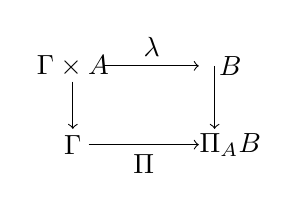
\begin{tikzpicture}
  \node at (0,1) {$\Gamma \times A$};
  \node at (2,1) {$B$};
  \node at (0,0) {$\Gamma$};
  \node at (2,0) {$\Pi_A B$};
  \draw[->] (0.4,1) -- node[above] {$\lambda$} (1.6,1);
  \draw[->] (0,0.8) -- (0,0.2);
  \draw[->] (1.8,1) -- (1.8,0.2);
  \draw[->] (0.2,0) -- node[below] {$\Pi$} (1.6,0);
\end{tikzpicture}

\subsection{$\Sigma$-Types}
For $\Gamma \vdash A : \text{Type}$ and $\Gamma, x : A \vdash B : \text{Type}$, the $\Sigma$-type $\Sigma_{x : A} B$ is formed via composition in the fibration.

The constructor $\text{pair}$ forms terms of $\Sigma_{x : A} B$. The pullback diagram is:

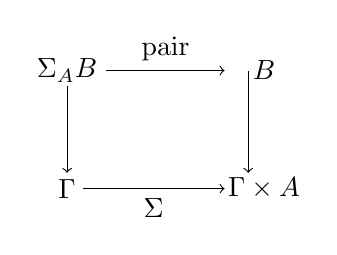
\begin{tikzpicture}
  \node at (0,1.5) {$\Sigma_A B$};
  \node at (2.5,1.5) {$B$};
  \node at (0,0) {$\Gamma$};
  \node at (2.5,0) {$\Gamma \times A$};
  \draw[->] (0.5,1.5) -- node[above] {$\text{pair}$} (2.0,1.5);
  \draw[->] (0,1.3) -- (0,0.2);
  \draw[->] (2.3,1.5) -- (2.3,0.2);
  \draw[->] (0.2,0) -- node[below] {$\Sigma$} (2.0,0);
\end{tikzpicture}

\subsection{Id-Types}
For $\Gamma \vdash A : \text{Type}$ and $a, b : A$, the identity type $\text{Id}_A(a, b)$ is formed using the diagonal map in the fibration.

The constructor $\text{refl}$ forms terms of $\text{Id}_A(a, a)$. The pullback diagram is:

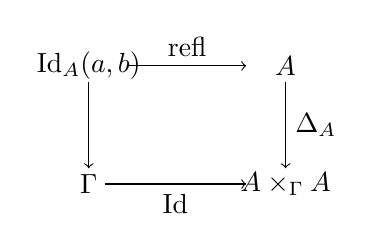
\begin{tikzpicture}
  \node at (0,1.5) {$\text{Id}_A(a, b)$};
  \node at (2.5,1.5) {$A$};
  \node at (0,0) {$\Gamma$};
  \node at (2.5,0) {$A \times_\Gamma A$};
  \draw[->] (0.5,1.5) -- node[above] {$\text{refl}$} (2.0,1.5);
  \draw[->] (0,1.3) -- (0,0.2);
  \draw[->] (2.5,1.3) -- node[right] {$\Delta_A$} (2.5,0.2);
  \draw[->] (0.2,0) -- node[below] {$\text{Id}$} (2.0,0);
\end{tikzpicture}

\newpage
\begin{lstlisting}[mathescape=true]
structure ComprehensionCategory (E B : Category) where
  fib : SplitFibration E B
  terminal : $\exists$ (T : B.Ob), $\forall$ (A : B.Ob), $\exists!$ (t : B.Hom A T), True
  comp_functor : $\forall$ (A : E.Ob), $\Sigma$ ($\Gamma$' : B.Ob) ($\pi$ : B.Hom $\Gamma$' (fib.functor.obj A))
  comp_adj : $\forall$ ($\Gamma$ : B.Ob) (A : E.Ob) (pA : fib.functor.obj A = $\Gamma$) ($\sigma$ : B.Hom $\Delta$ $\Gamma$),
    $\exists$ (A' : E.Ob) (pA' : fib.functor.obj A' = $\Delta$) (f : E.Hom A' A),
    fib.functor.map f = $\sigma$
  pullback : $\forall$ {A B C : B.Ob} (f : B.Hom A B) (g : B.Hom C B),
    $\exists$ (P : B.Ob) (h1 : B.Hom P A) (h2 : B.Hom P C),
    B.comp f h1 = B.comp g h2 $\wedge$
    $\forall$ (Q : B.Ob) (q1 : B.Hom Q A) (q2 : B.Hom Q C),
    B.comp f q1 = B.comp g q2 $\to$ $\exists$ (u : B.Hom Q P), B.comp h1 u = q1 $\wedge$ B.comp h2 u = q2
  pi : $\forall$ ($\Gamma$ : B.Ob) (A e : E.Ob) (f : E.Hom A e) (pA pe : fib.functor.obj A = $\Gamma$ $\wedge$ fib.functor.obj e = $\Gamma$),
    $\exists$ (Pi : E.Ob) (pi : E.Hom Pi $\Gamma$), fib.functor.obj Pi = $\Gamma$ $\wedge$
    $\forall$ (C : E.Ob) (g : E.Hom C A) (pC : fib.functor.obj C = $\Gamma$),
    $\exists$ (h : E.Hom C Pi), E.comp pi h = E.comp f g
  sigma : $\forall$ ($\Gamma$ : B.Ob) (A e : E.Ob) (f : E.Hom A e) (pA pe : fib.functor.obj A = $\Gamma$ $\wedge$ fib.functor.obj e = $\Gamma$),
    $\exists$ (Sigma : E.Ob) (sigma : E.Hom Sigma $\Gamma$), fib.functor.obj Sigma = $\Gamma$
  id : $\forall$ ($\Gamma$ : B.Ob) (A : E.Ob) (pA : fib.functor.obj A = $\Gamma$),
    $\exists$ (Id : E.Ob) (id : E.Hom Id A), fib.functor.obj Id = $\Gamma$

  Context : Type
  Context := B.Ob

  Type : Context $\to$ Type
  Type $\Gamma$ := $\Sigma$ (A : E.Ob), fib.functor.obj A = $\Gamma$

  Term : $\forall$ ($\Gamma$ : Context), Type $\Gamma$ $\to$ Type
  Term $\Gamma$ (A, pA) := $\Sigma$ (t : E.Hom $\Gamma$ A), fib.functor.map t = B.id

  ContextExt : $\forall$ ($\Gamma$ : Context), Type $\Gamma$ $\to$ Context
  ContextExt $\Gamma$ (A, pA) := (comp_functor A).1

  PiType : $\forall$ ($\Gamma$ : Context) (A : Type $\Gamma$), Type (ContextExt $\Gamma$ A) $\to$ Type $\Gamma$
  PiType $\Gamma$ (A, pA) (e, pe) := let res := pi $\Gamma$ A e E.id (pA, pe) in (res.1, res.2.1)

  SigmaType : $\forall$ ($\Gamma$ : Context) (A : Type $\Gamma$), Type (ContextExt $\Gamma$ A) $\to$ Type $\Gamma$
  SigmaType $\Gamma$ (A, pA) (e, pe) := let res := sigma $\Gamma$ A e E.id (pA, pe) in (res.1, res.2.1)

  IdType : $\forall$ ($\Gamma$ : Context) (A : Type $\Gamma$) (a b : Term $\Gamma$ A), Type $\Gamma$
  IdType $\Gamma$ (A, pA) (a, pa) (b, pb) := let res := id $\Gamma$ A pA in (res.1, res.2.1)
\end{lstlisting}

\newpage

\subsection{Conclusion}
The Lean 4 formalization provides a minimal, dependency-free model of MLTT-75 using a comprehension category, explicitly capturing type dependency and context extension via a Grothendieck fibration and comprehension functor. This contrasts with the representable maps approach, aligning more closely with traditional fibration-based models. The pullback diagrams, styled after Awodey, clarify the categorical constructions. Future work includes verifying the model with concrete examples and extending it to homotopy type theory.

\begin{thebibliography}{9}
\bibitem{jacobs1993}
Jacobs, B., ``Comprehension categories and the semantics of type dependency,'' TCS, 1993.
\bibitem{hofmann1997}
Hofmann, M., ``On the interpretation of type theory in locally cartesian closed categories,'' LFCS, 1997.
\bibitem{cartmell1986}
Cartmell, J., ``Generalised algebraic theories and contextual categories,'' APAL, 1986.
\bibitem{voevodsky2014}
Voevodsky, V., ``Notes on type systems,'' 2014.
\bibitem{awodey}
Awodey, S., ``Natural models of homotopy type theory,'' MSCS, 2018.
\end{thebibliography}

\end{document}
